\begin{figure}[!htb]
    \begin{center}
    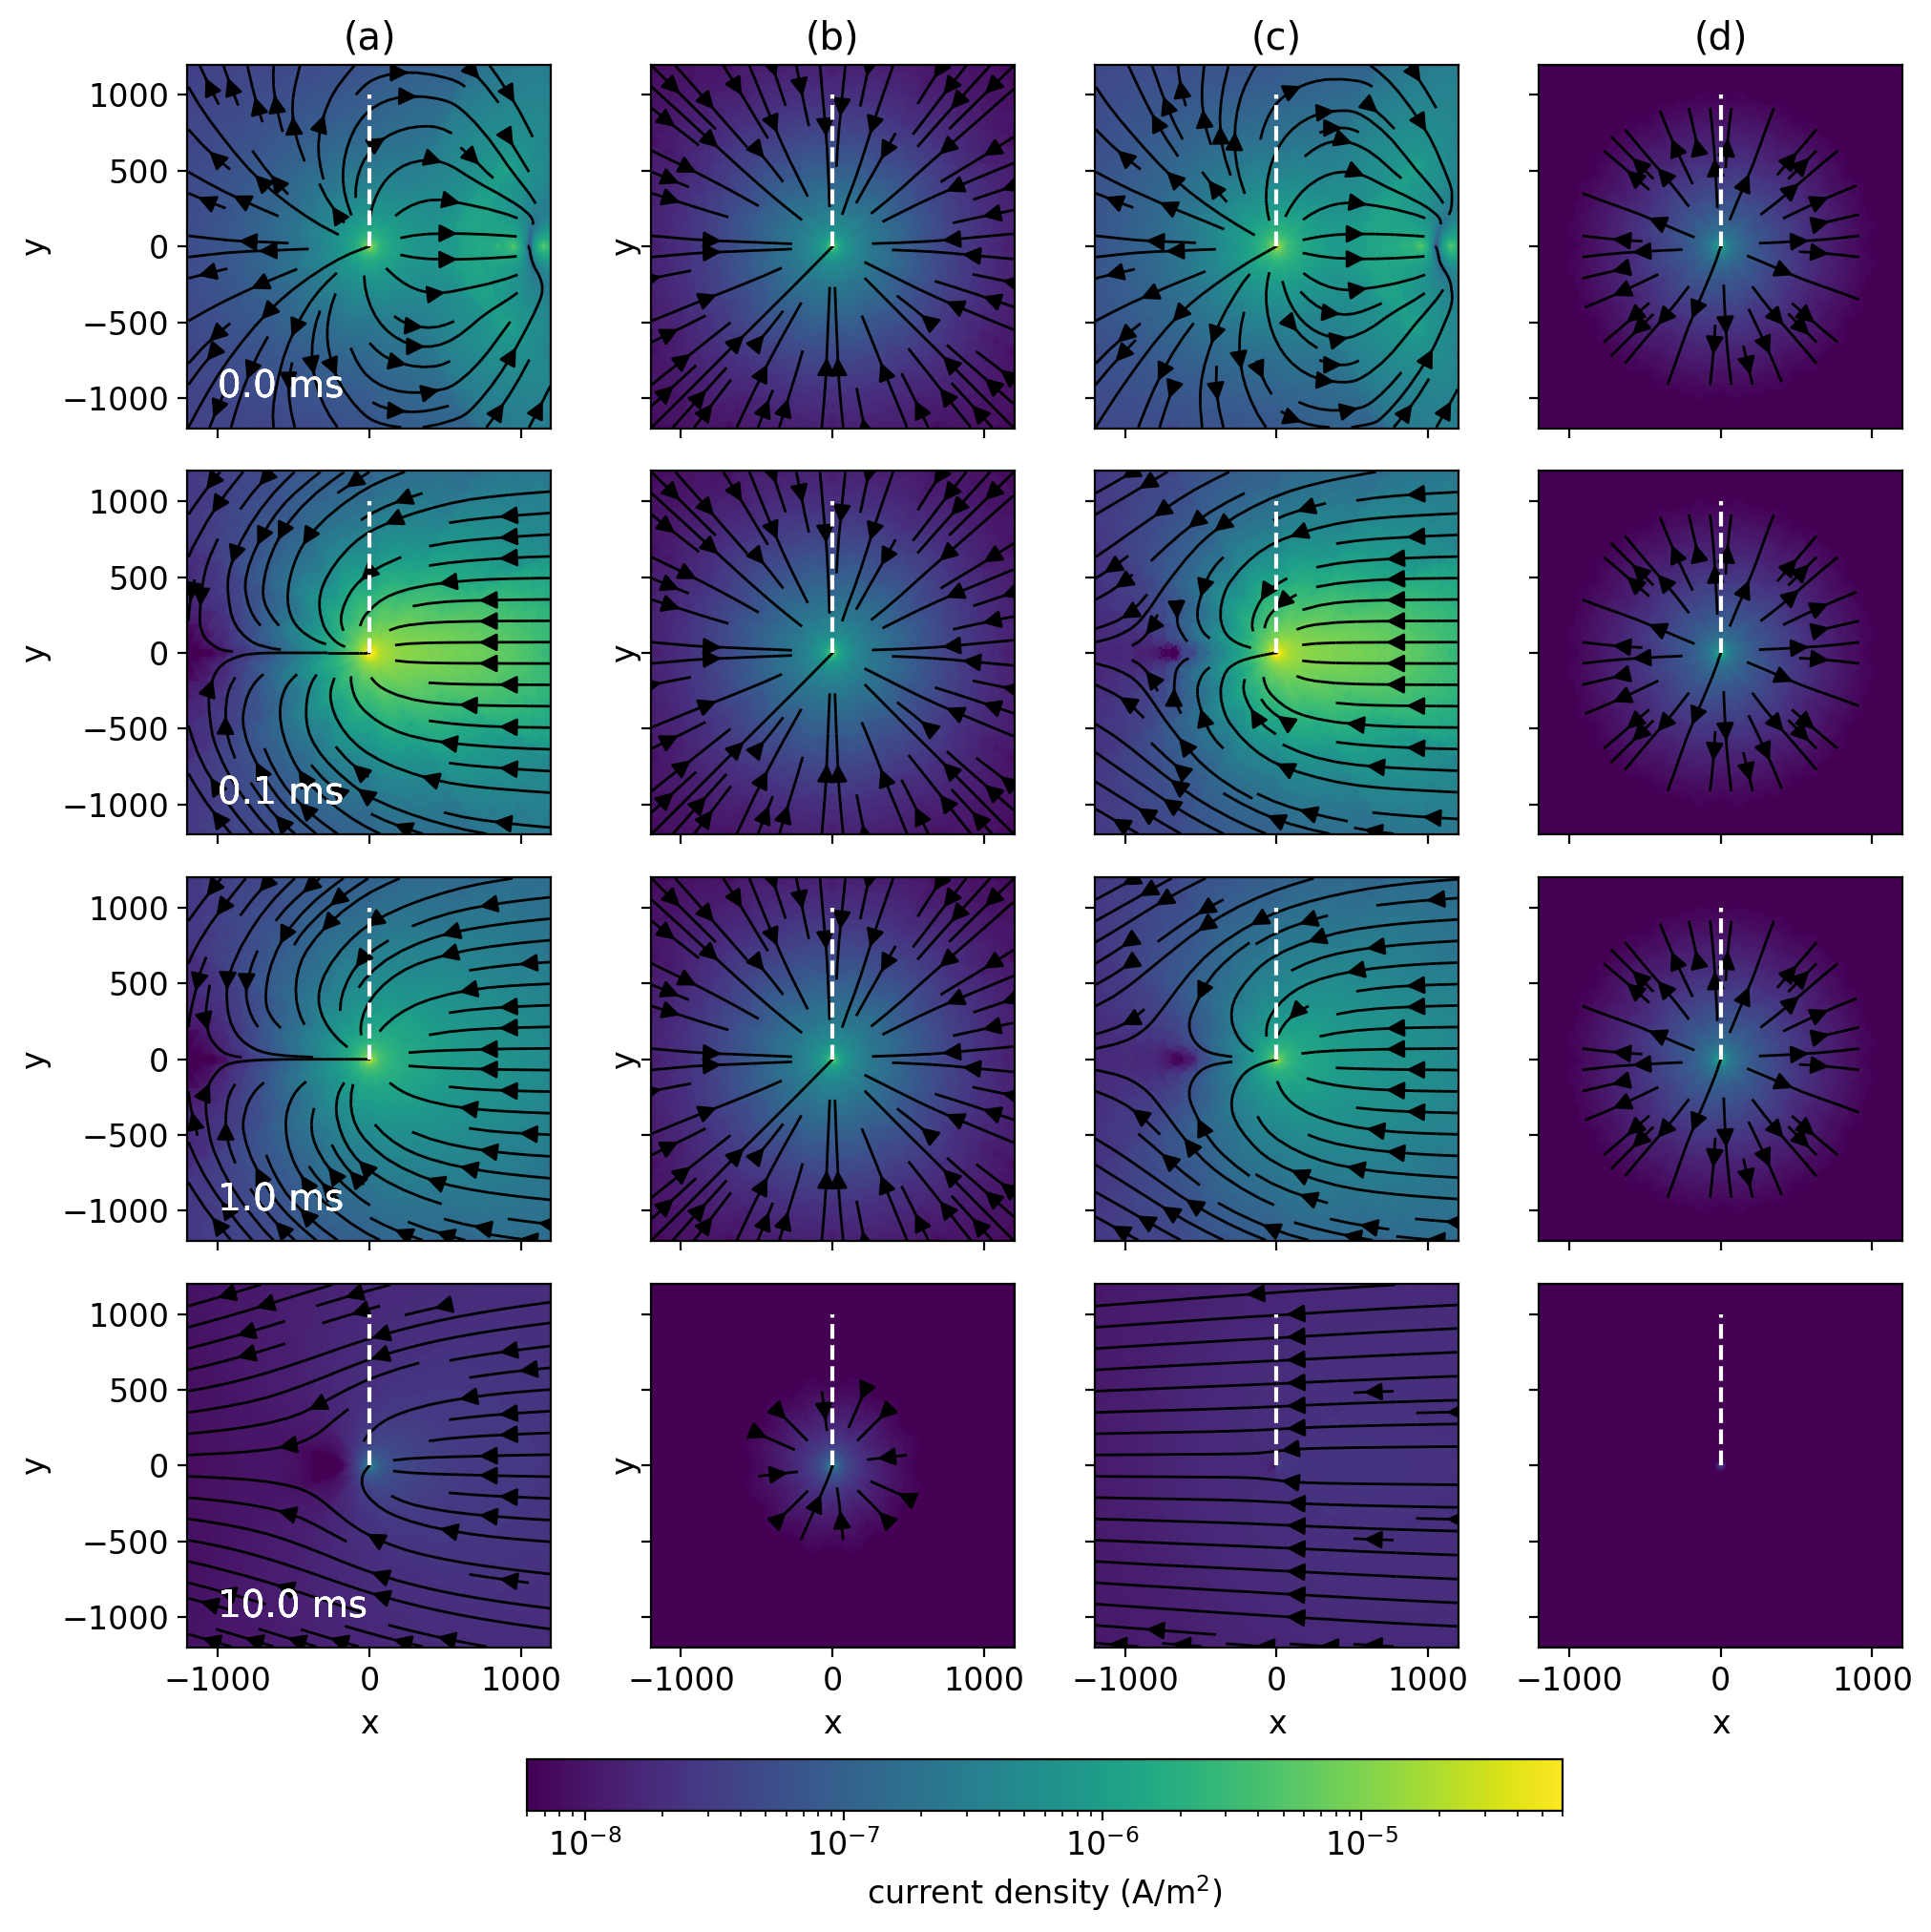
\includegraphics[width=1\textwidth]{figures/tdem-currents-depth-slice-target.png}
    \end{center}
\caption{
    Depth slices of the current density immediately below the surface ($z=-2.5$m) corresponding to the scenarios shown in Figure \ref{fig:tdem-currents-cross-section}: (a) current density for a conductive target in a halfspace with a conductive casing, (b) anomalous current density due to the conductive target, (c) current density for a resistive target with casing, and (d) anomalous current density due to the resistive target. The white dashed line indicates the survey line corresponsing to the electric field data shown in Figures \ref{fig:impact-of-wells-em-data} and \ref{fig:impact-of-wells-em-data-resistive}.
}
\label{fig:tdem-currents-depth-slice-target}
\end{figure}
